\section{Introduction}

The Metacognitive Profile Atlas is a public dataset of (answer, verbalized confidence) pairs from 33 frontier large language models (LLMs) on 1{,}500 stratified items from the Massive Multitask Language Understanding benchmark (MMLU; \citealp{hendrycks2021mmlu}). Items are grouped into six subject-group bins (Applied/Professional, Factual Recall, Formal Reasoning, Humanities/Comprehension, Natural Science, Social/Moral), 250 per bin. Models span eight families, including four Anthropic generations. After excluding parser-supplied values, the corpus holds 46{,}157 scored observations. Data are released under CC-BY-4.0 and code under MIT, with Croissant metadata.

\textbf{Why decompose by domain.} LLM confidence is used for abstention, routing and escalation \citep{wen2025}. Evaluations usually report one aggregate statistic, such as Type-2 AUROC (how well confidence separates correct from incorrect answers) or expected calibration error. An aggregate can hide domains where confidence carries little information. Gemini 2.5 Pro illustrates this. Its aggregate AUROC is .712, yet its confidence discriminates at .889 on Applied items and at chance (.485) on Natural Science items (\S\ref{sec:anomalous}).

\textbf{Background.} Type-2 AUROC is the standard nonparametric measure of metacognitive sensitivity in human research \citep{fleming2014,maniscalco2012}: the probability that a randomly chosen correct answer receives higher confidence than a randomly chosen error. It measures discrimination, not calibration. In LLMs, verbalized and token-based confidence carry some information about correctness \citep{kadavath2022}, but verbalized confidence is often overconfident and concentrated near the top of the scale \citep{xiong2023,yang2024}; \citet{steyvers2025} review the area. Selective prediction, which answers only above a confidence threshold, depends on discrimination \citep{elyaniv2010,geifman2017}. Mechanistic work suggests verbal confidence reflects a distinct internal evaluation \citep{kumaran2026}, separable from calibration directions in the residual stream \citep{miao2026}. Hidden-state signatures of known versus unknown items are also reported \citep{kim2026}. \citet{haznitrama2026} profile capability across many models. The atlas asks a narrower question: whether confidence discrimination differs systematically across content domains, across many models, on one benchmark.

\textbf{Contributions.}
\begin{enumerate}
\item A 33-model dataset of item-level answers and verbalized confidence on 1{,}500 stratified MMLU items, with per-cell error counts, bootstrap intervals, parsing code and an item locator table.
\item A population-level ordering on MMLU: Applied/Professional is the domain where confidence discriminates best, and Formal Reasoning and Natural Science are where it discriminates worst. The ordering survives precision weighting, bootstrap rank analysis and Holm-corrected pairwise tests. The middle domains are not distinguishable.
\item Evidence about what is \emph{not} reliable: per-model six-domain profiles have weak split-half reliability, and the six bins do not form cohesive subject groups. Per-model profiles and family patterns are released as exploratory.
\item A paired-item decomposition showing that equal aggregate gains between model generations can come from opposite mechanisms: genuine monitoring improvement or error removal.
\end{enumerate}

The atlas is a benchmark-stage description on MMLU, not a deployment certification. All claims are specific to MMLU and to one verbalized-confidence prompt.

\section{Methods}

\textbf{Models and items.} Thirty-three LLMs from eight families were evaluated through the Kaggle Benchmarks platform (March--April 2026). The families were Anthropic (Opus 4.1--4.7, Sonnet 4--4.6, Haiku 4.5; $n=8$), DeepSeek (V3.1, V3.2, R1; $n=3$), Google-Gemini (2.0 Flash through 3.1 Pro; $n=7$), Google-Gemma (3 1B through 4 31B; $n=5$), OpenAI (GPT-5.4 nano, mini and full, GPT-oss-20B and 120B; $n=5$), Qwen ($n=4$) and Zhipu (GLM-5). All calls used greedy decoding (temperature 0) and an independent conversation per item. Items are 1{,}500 MMLU test questions drawn deterministically (seed 42), 250 per bin. Fifty-six of 57 MMLU subjects were mapped a priori to the six bins. \texttt{college\_medicine} was left unmapped because it is ambiguous between Natural Science and Applied/Professional. (Version 1 named the excluded subject as \texttt{elementary\_mathematics}, which is in fact mapped to Formal Reasoning.) Table~\ref{tab:domains} summarises the bins. A per-observation (subject, split, row-index) locator table is released.

\begin{table}[!htbp]
\centering
\caption{MMLU-to-domain mapping (partial). Full mapping in the repository.}
\label{tab:domains}
\small
\begin{tabular}{llrr}
\toprule
\textbf{Domain bin} & \textbf{Label} & \textbf{Available items} & \textbf{Sampled} \\
\midrule
Applied/Professional & Applied & 3{,}610 & 250 \\
Factual Recall & Factual & 2{,}998 & 250 \\
Formal Reasoning & Formal & 1{,}910 & 250 \\
Humanities/Comprehension & Human. & 987 & 250 \\
Natural Science & Science & 1{,}532 & 250 \\
Social/Moral & Social & 2{,}832 & 250 \\
\bottomrule
\end{tabular}
\end{table}

\textbf{Elicitation and parsing.} Each item was presented as multiple choice (A--D). The model was asked for its answer and a confidence from 0 to 100 in a fixed format, with no chain-of-thought cue (Appendix~\ref{app:prompt}). Answers and confidences were extracted by a documented rule hierarchy (Appendix~\ref{app:parsing}). Two kinds of record are excluded before analysis. The first is unparsed answers (13 records across six models). The second is confidence values the parser supplied because none could be extracted: the parser substituted 50, and 980 of the 985 such records belong to GPT-oss-120B, which never states 50 itself. The other five are in four models. In every affected model no response genuinely states a confidence of 50, so all its 50s can be identified as parser defaults. These values describe the pipeline, not the model, and including them in version 1 manufactured an apparently anomalous profile for GPT-oss-120B. After exclusion, 46{,}157 observations remain. Sixteen models have fewer than 1{,}500 scored items: twelve because of platform timeouts during the run (the smallest is GLM-5 with 598) and four because of the exclusions. GPT-oss-120B retains 518 items.

\textbf{Analysis.} Type-2 AUROC was computed per model and per model-domain cell from the raw 0--100 confidence. Bootstrap 95\% intervals used 1{,}000 resamples per cell, each cell seeded separately so that its interval depends only on its own data, and per-cell error counts are reported (Table~\ref{tab:s1}). The domain ordering was tested with Friedman's test and Kendall's $W$ over the 33 models. Robustness was checked in four ways: excluding wide-interval or few-error cells, inverse-variance weighting, bootstrap rank stability (500 item resamples within every cell), and Holm-corrected Wilcoxon contrasts for all 15 domain pairs. Ipsative profiles subtract each model's own mean across domains. Family similarity of profile shape compares within-family and between-family correlations of ipsative profiles by permutation (10{,}000 shuffles), with per-family tests Holm-corrected.

\section{Results}

\textbf{Dataset summary.} Accuracy ranges from .388 (Gemma 3 1B) to .951 (Opus 4.6, Gemini 3 Flash). Aggregate AUROC ranges from .498 (Gemma 3 1B) to .806 (Opus 4.6). The 198 model-domain cells have a median of 20 errors (minimum 2; 28 cells have fewer than 10). Their bootstrap intervals have median width .202; 36\% are wider than .25, mostly in high-accuracy models where few errors leave the estimate unstable. Table~\ref{tab:matrix} gives the full matrix and Figure~\ref{fig:heatmap} the heatmap.

\begin{figure}[!htbp]
\centering
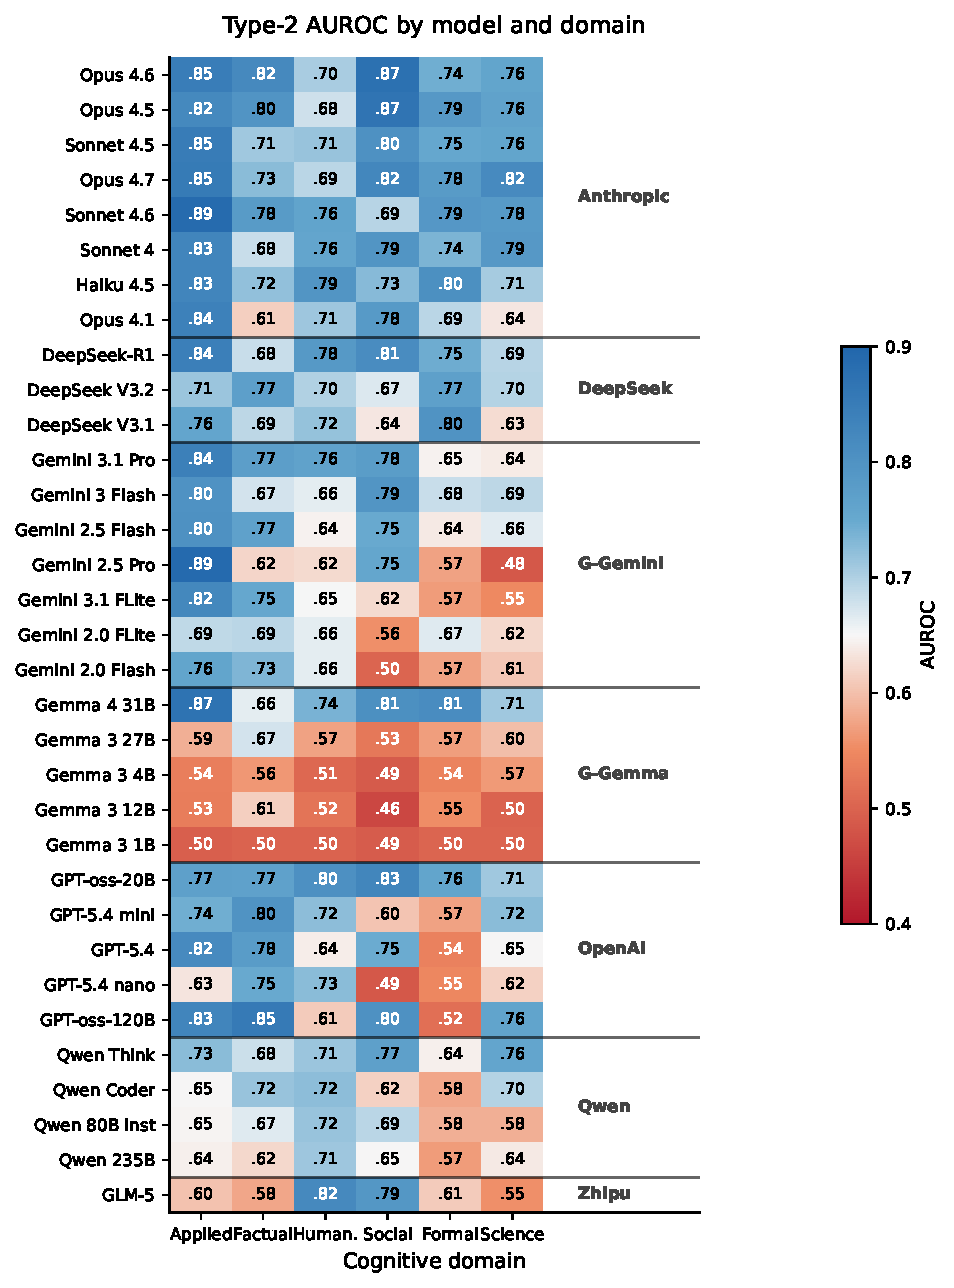
\includegraphics[width=0.78\textwidth]{fig1_heatmap.pdf}
\caption{Type-2 AUROC by model (rows) and MMLU domain bin (columns). The colour scale spans .40 to .90, so its visual midpoint is about .65, not chance (.50). Family separators are horizontal lines. Full values: Table~\ref{tab:matrix}; intervals and error counts: Table~\ref{tab:s1}.}
\label{fig:heatmap}
\end{figure}

\subsection{Domain ordering}
\label{sec:hierarchy}

Confidence discriminates best on Applied items and worst on Formal and Science items (Table~\ref{tab:hierarchy}, Figure~\ref{fig:hierarchy}; Friedman $\chi^2(5) = 28.26$, $p < .0001$; Kendall's $W = .171$). Applied ranks in the top two within 21 of 33 models, and Formal or Science occupies a bottom-two rank in 27 of 33. The low concordance means models agree on the extremes, not on the middle.

\begin{table}[!htbp]
\centering
\caption{Domain means across 33 models (Type-2 AUROC).}
\label{tab:hierarchy}
\small
\begin{tabular}{llrrrrr}
\toprule
\textbf{Rank} & \textbf{Domain} & \textbf{Mean AUROC} & \textbf{SD} & \textbf{Mean rank} & \textbf{\#1 in} & \textbf{Last in} \\
\midrule
1 & Applied & .750 & .112 & 2.09 & 15/33 & 0/33 \\
2 & Factual & .703 & .079 & 3.33 & 7/33 & 5/33 \\
3 & Social & .697 & .124 & 3.48 & 4/33 & 9/33 \\
4 & Humanities & .688 & .080 & 3.73 & 4/33 & 4/33 \\
5 & Science & .662 & .089 & 4.21 & 1/33 & 8/33 \\
6 & Formal & .655 & .100 & 4.15 & 2/33 & 7/33 \\
\bottomrule
\end{tabular}
\end{table}

\begin{figure}[!htbp]
\centering
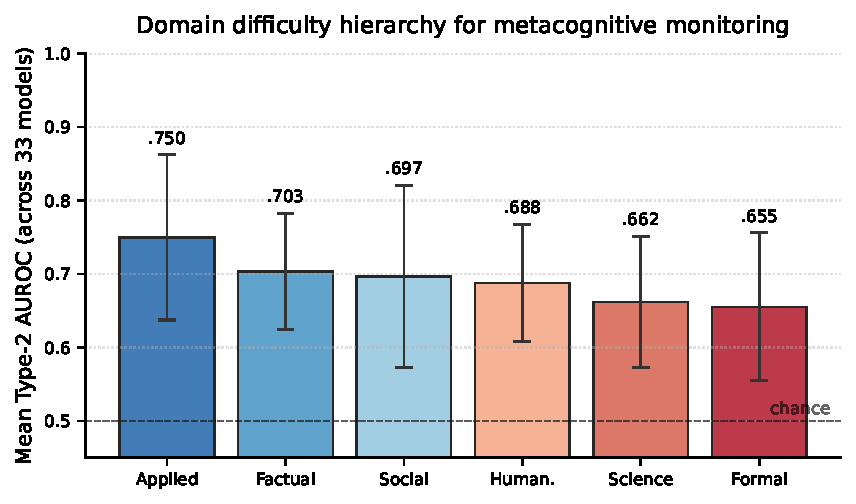
\includegraphics[width=0.7\textwidth]{fig2_domain_hierarchy.pdf}
\caption{Mean Type-2 AUROC per domain across 33 models, with standard deviation bars.}
\label{fig:hierarchy}
\end{figure}

\textbf{Robustness.} The ordering does not depend on imprecise cells (Table~\ref{tab:precision}). Applied stays first and Formal and Science stay in the bottom two under every exclusion rule and under inverse-variance weighting. Under the exclusions, concordance rises ($W$ = .20 to .32), although the Friedman test then rests on fewer complete models. In 500 bootstrap resamples of items within every cell, Applied ranks first in 100\% of resamples, Formal falls in the bottom two in 93\% and Science in 92\%. The gap between Applied and the lowest domain is .098 (95\% interval [.073, .129]). Holm-corrected Wilcoxon tests over the 15 domain pairs show Applied exceeding Formal, Science, Social and Humanities ($p_{\text{Holm}} \le .011$). No other pair survives correction, including Applied versus Factual ($p_{\text{Holm}} = .14$) and Formal versus Science ($p = .87$). Applied is the one reliably distinct domain; Formal and Science form an undifferentiated bottom pair.

\begin{table}[!htbp]
\centering
\caption{Domain ordering under precision-based variants. Friedman tests use only models with all six cells retained.}
\label{tab:precision}
\footnotesize
\setlength{\tabcolsep}{3.5pt}
\begin{tabular}{lrcccccc}
\toprule
\textbf{Variant} & \textbf{Cells} & \textbf{Applied} & \textbf{Formal} & \textbf{Science} & \textbf{Models} & \textbf{Friedman} & \textbf{$W$} \\
\midrule
All cells & 198 & .750 (1st) & .655 (6th) & .662 (5th) & 33 & $\chi^2 = 28.26$, $p < .0001$ & .171 \\
CI width $\le .30$ & 157 & .754 (1st) & .615 (6th) & .659 (5th) & 15 & $\chi^2 = 16.94$, $p = .005$ & .226 \\
CI width $\le .25$ & 127 & .754 (1st) & .586 (6th) & .623 (5th) & 10 & $\chi^2 = 15.83$, $p = .007$ & .317 \\
$\ge 10$ errors & 170 & .754 (1st) & .642 (6th) & .672 (5th) & 18 & $\chi^2 = 18.03$, $p = .003$ & .200 \\
Inverse-variance weighted & 198 & .711 (1st) & .572 (5th) & .534 (6th) & -- & -- & -- \\
\bottomrule
\end{tabular}
\end{table}

\textbf{Accuracy.} The ordering is not explained by domain difficulty in any simple way. Applied has the \emph{lowest} mean accuracy (.828) and Humanities the highest (.922). Across the six domains, mean accuracy and mean AUROC correlate negatively ($\rho = -.31$), and within models the centred correlation is $r = .01$. These checks rule out a monotonic accuracy confound, not every effect of item composition. In high-accuracy cells AUROC rests on few errors, and that sparse-error regime is what the precision analyses address.

\textbf{Reliability: the extremum is reliable, the profile is not.} Aggregate AUROC is reproducible across random item halves (cross-model $r = .868$). The population-level contrast between Applied and the mean of Formal and Science has a split-half correlation across models of .249 (median over 50 splits; IQR .162--.343; Spearman--Brown .40), and its sign is positive in both halves in 50 of 50 splits. Full six-domain profile shapes within a model are much less reliable. Across the same splits the median correlation between halves is .157 (Spearman--Brown .27). Over 100 splits the grand median of per-model medians is .076, and 58\% of models are positive. That last figure is sensitive to individual models because per-model values are spread thinly around it. The claims of this paper therefore rest on the population-level ordering; per-model profiles are released for exploration and should be read against their intervals.

\textbf{Domain bins are not cohesive.} Correlations of per-subject AUROC across models are no higher between subjects in the same bin than between subjects in different bins (mean $r = .173$ in both cases). The bins group MMLU subjects by pragmatic content, not by an empirically cohesive construct. The same limitation shows at the subject level. Applied subjects rank higher on average than Formal and Science subjects (mean rank 19.6 versus 28.8 and 21.1 of 47), but the difference is not significant (Mann--Whitney $p = .18$).

\subsection{Families and generations (exploratory)}

Family-level aggregate AUROC ranges from .573 (Gemma) to .777 (Anthropic) (Table~\ref{tab:families}). Anthropic is the most consistent family (.708--.806 across eight models). In OpenAI, the two open-weight GPT-oss models (.793 and .800) exceed GPT-5.4 (.649), mini (.651) and nano (.582). Version 1 attributed OpenAI's spread to GPT-oss-120B's low AUROC and inferred that training recipe dominates scale; that inference rested on the imputed values and is withdrawn.

\begin{table}[!htbp]
\centering
\caption{Family-level aggregate Type-2 AUROC.}
\label{tab:families}
\small
\begin{tabular}{lrrr}
\toprule
\textbf{Family} & \textbf{\# models} & \textbf{Mean AUROC} & \textbf{Range} \\
\midrule
Anthropic & 8 & .777 & .708--.806 \\
DeepSeek & 3 & .740 & .716--.769 \\
Zhipu & 1 & .697 & -- \\
OpenAI & 5 & .695 & .582--.800 \\
Google-Gemini & 7 & .693 & .623--.765 \\
Qwen & 4 & .669 & .621--.745 \\
Google-Gemma & 5 & .573 & .498--.771 \\
\bottomrule
\end{tabular}
\end{table}

\textbf{Profile-shape similarity within families.} Ipsative profiles correlate more within families than between them: the mean within-family $r$ is .406 against .091 between, a difference of .316 (permutation $p = .0001$). Per family, only Anthropic is individually supported after Holm correction (Table~\ref{tab:family}). Gemini and Qwen are nominally significant and are reported as exploratory patterns. Given the weak reliability of individual profiles, these family patterns should be treated with the same caution. Figure~\ref{fig:ipsative} shows the profiles.

\begin{table}[!htbp]
\centering
\caption{Per-family permutation tests of profile-shape similarity (10{,}000 permutations; statistic = within-family minus between-family mean correlation), Holm-corrected across six families. Zhipu ($n = 1$) is not testable.}
\label{tab:family}
\small
\begin{tabular}{lrrrrrr}
\toprule
\textbf{Family} & \textbf{$n$} & \textbf{Within $r$} & \textbf{Between $r$} & \textbf{Statistic} & \textbf{$p$} & \textbf{$p_{\text{Holm}}$} \\
\midrule
Anthropic & 8 & .446 & .085 & .360 & .003 & .019 \\
Qwen & 4 & .482 & .025 & .458 & .018 & .092 \\
Google-Gemini & 7 & .511 & .232 & .279 & .019 & .092 \\
Google-Gemma & 5 & .210 & $-$.046 & .256 & .066 & .197 \\
OpenAI & 5 & .310 & .156 & .154 & .155 & .310 \\
DeepSeek & 3 & .125 & .065 & .060 & .370 & .370 \\
\bottomrule
\end{tabular}
\end{table}

\begin{figure}[!htbp]
\centering
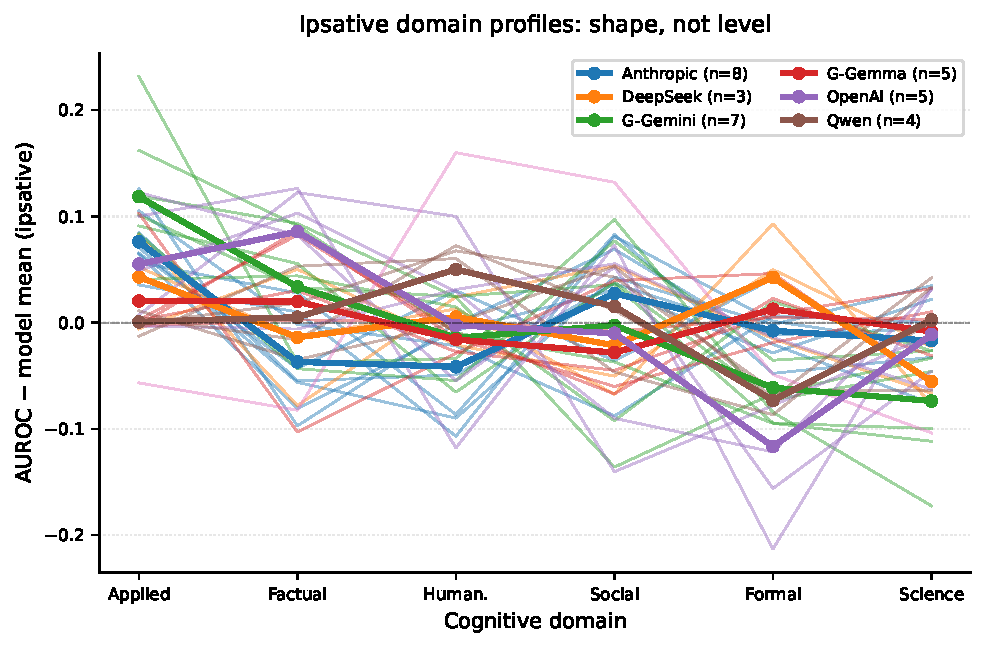
\includegraphics[width=0.78\textwidth]{fig3_ipsative.pdf}
\caption{Ipsative domain profiles for all 33 models, coloured by family (thin lines: models; bold: family means). Centring on each model's mean isolates profile shape from level. Individual profiles are not reliable (\S\ref{sec:hierarchy}) and are shown for exploration.}
\label{fig:ipsative}
\end{figure}

\textbf{Generational change: monitoring gain versus error removal.} Aggregate AUROC rises across several model generations (Figure~\ref{fig:generational}). The Opus line goes from .708 (4.1) to .798 (4.5) and then stays flat (.806, .792) despite continued accuracy gains. Gemma 3 27B (.565) to Gemma 4 31B (.771) is the largest single step. A higher AUROC can arise in two ways: the newer model doubts errors it still makes (better monitoring), or it stops making the confidently wrong answers that depressed the older model's AUROC (error removal). Table~\ref{tab:generational} separates the two on the items the earlier model answered wrongly with confidence of at least 70.

\begin{table}[!htbp]
\centering
\caption{Paired-item decomposition on items the earlier model answered wrongly with confidence $\ge 70$. ``Fixed'': share answered correctly by the later model. $\Delta$conf: mean change in confidence on items still wrong (Wilcoxon signed-rank).}
\label{tab:generational}
\footnotesize
\setlength{\tabcolsep}{4pt}
\begin{tabular}{lrrrrl}
\toprule
\textbf{Pair} & \textbf{Items} & \textbf{Fixed} & \textbf{$\Delta$conf (still wrong)} & \textbf{$p$} & \textbf{Reading} \\
\midrule
Gemma 3 27B $\to$ Gemma 4 31B & 321 & 82.6\% & $-$2.7 & .052 & Error removal \\
Opus 4.1 $\to$ Opus 4.5 & 80 & 35.0\% & $-$7.9 & $3.1\times10^{-7}$ & Monitoring gain \\
Opus 4.1 $\to$ Opus 4.7 & 80 & 45.0\% & $-$6.6 & $3.3\times10^{-5}$ & Monitoring gain \\
Opus 4.5 $\to$ Opus 4.7 & 66 & 37.9\% & $+$0.2 & .59 & Neither \\
DeepSeek V3.1 $\to$ V3.2 & 160 & 37.5\% & $-$2.0 & .002 & Weak monitoring gain \\
DeepSeek V3.2 $\to$ R1 & 135 & 47.4\% & $-$1.8 & .28 & Error removal \\
\bottomrule
\end{tabular}
\end{table}

The Gemma step is mainly error removal. Gemma 4 answers 82.6\% of those items correctly, its confidence on them rises (94.8 to 97.2), and on its 32 newly wrong items it reports a mean confidence of 90.8. The Opus steps show the signature of better monitoring. Opus 4.5 lowers its confidence on the errors that persist (89.1 to 81.2) and even on the errors it fixes (85.7 to 77.9), and Opus 4.7's 31 newly wrong items carry a mean confidence of only 71.5. Similar aggregate gains can therefore come from opposite mechanisms, which is the main reason for releasing paired item-level data. Gemma 3 1B's domain intervals are the narrowest in the atlas (all widths at most .06), so its near-chance aggregate (.498) is a precise estimate of absent discrimination, not noise.

\begin{figure}[!htbp]
\centering
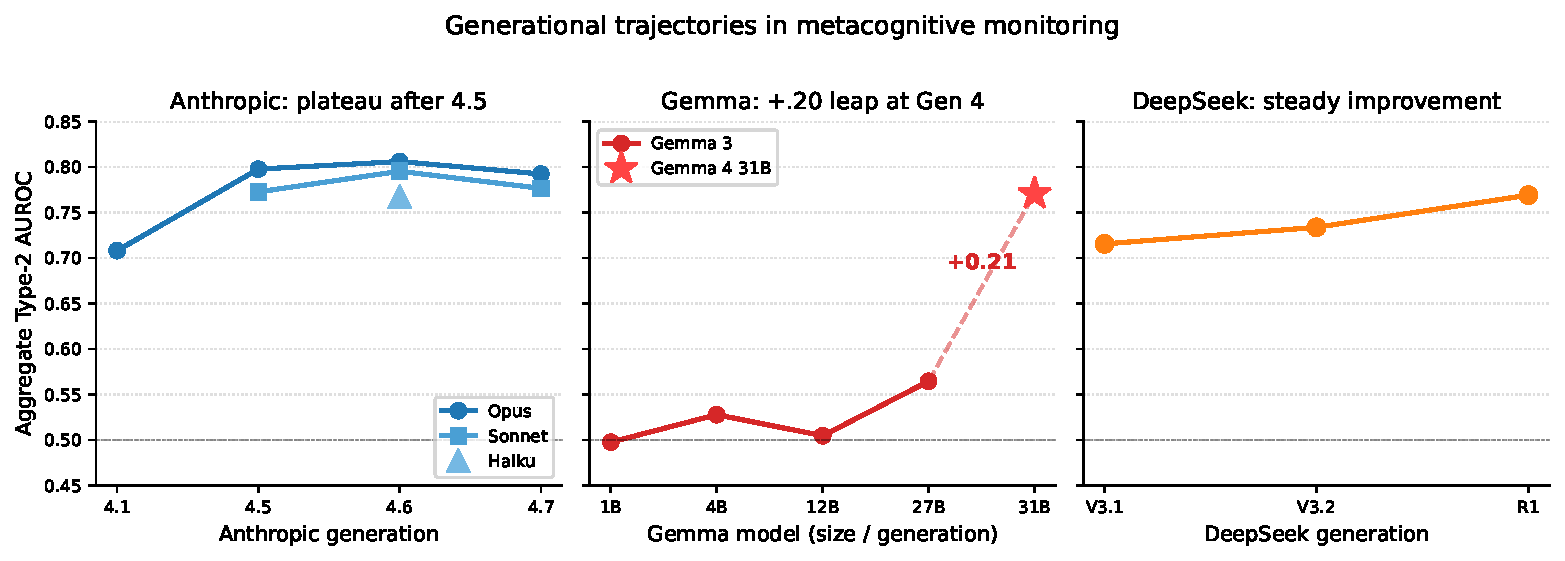
\includegraphics[width=\textwidth]{fig5_generational.pdf}
\caption{Aggregate Type-2 AUROC across generations for Anthropic, Gemma and DeepSeek. Table~\ref{tab:generational} decomposes the changes.}
\label{fig:generational}
\end{figure}

\subsection{Binary-probe validity screening and verbalized confidence}
\label{sec:probe}

Twenty of the 33 models were also tested on a separate 524-item battery that asks after each answer whether to KEEP or WITHDRAW it \citep{cacioli2026c}. A portable validity screen \citep{cacioli2026e} classifies a binary confidence signal from the correctness-by-confidence table. It is Invalid when a response set is established: confidence kept on at least 95\% of errors (L), or withdrawn on at least half of correct answers (Fp), with interval guards. It is Indeterminate when such a pattern cannot be certified, often because there are too few errors, or when confidence does not measurably track correctness. It is Valid otherwise. The corrected classification (arXiv:2604.17714v2) uses the battery's five keyed tracks. It finds DeepSeek-R1 Invalid: it withdraws 95\% of its correct answers, and with only six errors whether its withdrawals track correctness cannot be assessed. Gemini 3.1 Pro and Qwen3 Next 80B Thinking are Indeterminate: they keep confidence on 96\% of their errors but make 24 and 27 errors, too few to certify blanket confidence. Gemini 3 Flash and GPT-5.4 nano are also Indeterminate, with no detectable item sensitivity. Version 1 of this paper described R1 as showing catastrophic inversion; that description came from a scoring error in the battery analysis and is withdrawn.

Under verbalized confidence the picture differs in both directions (Figure~\ref{fig:cross}). R1, Gemini 3.1 Pro and Qwen Thinking discriminate well on MMLU (aggregate AUROC .769, .765 and .745; domain ranges .682--.843, .640--.841 and .644--.768). Gemma 3 1B, 12B and 27B are Valid on the binary battery, yet their verbalized confidence barely discriminates on MMLU (.498, .505 and .565). Across the 20 models, battery AUROC does not predict atlas AUROC (Spearman $\rho = .00$). Screened on MMLU at a cut point of 90 (confidence $\ge 90$ counts as high), the four Gemma 3 models are Invalid, Gemini 2.5 Pro is Indeterminate, and the other 28 are Valid. A model's confidence quality is therefore specific to the probe format and task under which it is measured. A binary-probe result says little about verbalized confidence on another benchmark, and the reverse.

\begin{figure}[!htbp]
\centering
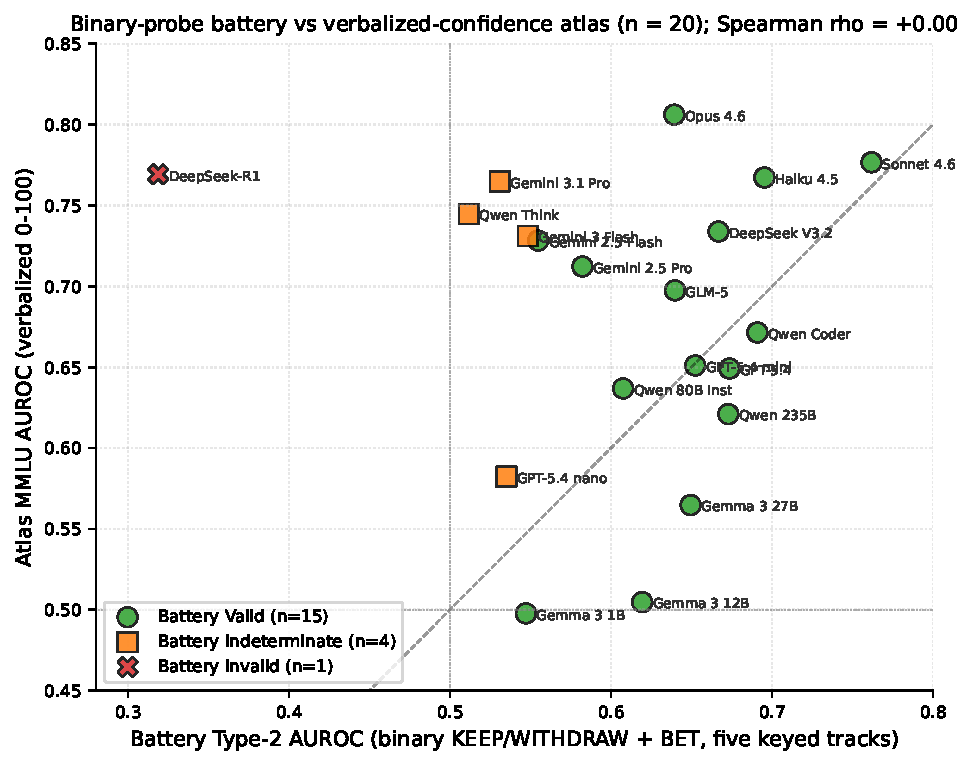
\includegraphics[width=0.72\textwidth]{fig7_cross_benchmark.pdf}
\caption{Battery Type-2 AUROC (binary KEEP/WITHDRAW + BET probes, five keyed tracks; \citealp{cacioli2026e}) against atlas aggregate AUROC (verbalized 0--100 confidence on MMLU) for the 20 models in both. Markers show the corrected battery tier. The dashed line is identity.}
\label{fig:cross}
\end{figure}

\subsection{Individual profiles}
\label{sec:anomalous}

These descriptions are exploratory (\S\ref{sec:hierarchy}).

\textbf{Gemini 2.5 Pro} has the widest within-model spread: Applied .889 [.794, .960], Science .485 [.470, .497], Formal .573 [.478, .778]. The Applied lower bound exceeds the Science upper bound, so the difference is not sampling noise. The aggregate (.712) gives no sign that its Science-domain confidence is at chance. This run is partial (981 items).

\textbf{GLM-5} is the only model whose Humanities AUROC (.818 [.706, .972]) is well above its Applied AUROC (.602). Its run is partial (598 items), and its Humanities estimate rests on three errors. A complete rerun three months later shows what can and cannot be concluded. On the 598 items common to both runs, correctness agreed on 98.5\% of items, item-level confidence correlated $r = .71$, and the six-domain ordering correlated $\rho = .77$ ($p = .072$, six domains). Humanities again exceeded Applied (.792 versus .639), and the aggregate AUROC rose from .697 to .759. The rerun's errors per domain numbered between 2 and 12, so its domain estimates are imprecise as well (Appendix~\ref{app:glm5}).

\textbf{GPT-oss-120B.} Version 1 reported this model as having the highest confidence variability in the atlas with near-chance discrimination (SD 21.3, AUROC .530), and offered it as a distinct failure mode. That profile was produced by 980 parser-imputed values of 50. On its 518 genuine responses its aggregate AUROC is .800 and its domain values range from .515 (Formal) to .855 (Factual). Its imputation rate also differs by domain (59\% to 74\%; $\chi^2(5) = 18.67$, $p = .002$), so the retained items are not a random sample. With 65 to 102 items per domain and wide intervals (Formal: [.128, .918]), its profile should not be interpreted.

\subsection{Validation summary}
\label{sec:coherence}

Aggregate AUROC rankings are reproducible on half the items ($r = .868$; Appendix Figure~\ref{fig:splithalf}). The population-level extremum contrast is reproducible in sign but modest in reliability. Per-model profiles are not reliable, and the domain bins are not cohesive (\S\ref{sec:hierarchy}). The paper's claims are limited accordingly.

\section{Discussion}

\textbf{What the atlas shows.} On MMLU, verbalized confidence across 33 frontier models discriminates correct from incorrect answers best on applied professional knowledge and worst on formal reasoning and natural science. The pattern holds at the population level under precision weighting, bootstrap rank analysis and multiplicity-corrected contrasts. One plausible account: Applied items (law, medicine, accounting) tend to have answers anchored in specific retrieved knowledge, so whether a model knows the answer may leave a clearer internal trace. Formal items admit plausible intermediate steps that end at wrong answers. This fits the hypothesis of \citet{kim2026} that well-learned factual material produces more separable internal states. Nothing here examines hidden states, so the account is a hypothesis, not a mechanism.

\textbf{What it does not show.} It does not show that any individual model has a stable domain profile: per-model profiles have weak split-half reliability. It does not show that the six bins are cognitive constructs: subjects within a bin are no more alike than subjects across bins. It does not show that the ordering holds beyond MMLU or beyond this prompt; replication on a benchmark with non-overlapping items (for example GPQA) is the necessary next test. Type-2 AUROC measures discrimination, not calibration.

\textbf{Implications for confidence-based abstention.} If a deployment applies one confidence threshold across content types, the population-level result predicts that the threshold will be less informative on formal and scientific content than on applied professional content. This argues for checking discrimination separately on the content a system will see, rather than relying on a single aggregate. It does not support looking up a particular model's domain profile in this atlas and treating it as reliable. In flagship models, adjacent-domain differences are not interpretable at current item counts: GPT-5.4's Formal AUROC is .539 [.452, .631], for example. Those comparisons need many more errors per cell.

\textbf{Probe format.} Classifications from a binary KEEP/WITHDRAW probe did not predict discrimination under verbalized confidence, in either direction (\S\ref{sec:probe}). Statements about a model's confidence should name the probe and task: ``no detectable signal under probe X on task Y'', not ``no signal''.

\textbf{Parsing is part of the measurement.} The largest correction in this version came from parser-supplied values being treated as model output. Releasing raw outputs, extraction code and per-model fallback counts made the error findable. We recommend that verbalized-confidence datasets report imputation and fallback rates per model, and exclude imputed values before analysis.

\textbf{Limitations.} The results cover MMLU only and one verbalized-confidence prompt, with greedy decoding. The domain mapping is a priori and not empirically cohesive. Per-cell estimates are imprecise for high-accuracy models, with 36\% of intervals wider than .25 and 28 cells with fewer than 10 errors. Sixteen runs are partial (twelve from platform timeouts, four from exclusions), and GPT-oss-120B's retained items are a non-random subset. Answers and confidences were extracted by rules, with fallbacks that can occasionally capture an unintended letter or number (Appendix~\ref{app:parsing}). No causal mechanism is tested.

\section{Conclusion}

Aggregate confidence metrics hide a reliable population-level pattern on MMLU: verbalized confidence in frontier models discriminates best on applied professional knowledge and worst on formal reasoning and natural science. Per-model profiles are too unreliable to interpret individually at this item count. The atlas releases the item-level data, error counts, parsing code and locators needed to test these patterns on other benchmarks and probes.

\section*{Open science}

Data (item-level CSVs, error counts, bootstrap intervals, MMLU locators, parsing fallback counts), extraction and analysis code, and a single script that regenerates every number and figure are at \url{https://github.com/synthiumjp/metacognitive-profile-atlas} (MIT, code) and \url{https://huggingface.co/datasets/synthiumjp/metacognitive-profile-atlas} (CC-BY-4.0, data; Croissant metadata).

\section*{Use of AI}

Claude (Anthropic) assisted with benchmark design, analysis code and manuscript preparation. Analysis code was checked against \texttt{scikit-learn} reference implementations and by re-running the full pipeline from raw data; the corrections in this version were found by such re-analysis. All scientific decisions, the domain mapping and the interpretations are the author's.
